\chapter{जैव-भू-रासायनिक चक्र}\label{ch:b2:biogeochemical-cycles}

मार्च 1958 में चार्ल्स कीलिंग नाम के किसी युवा रसायनज्ञ ने हवाई के
मौना लोआ की उत्तरी ढलान पर, प्रशांत से साढ़े तीन किलोमीटर ऊपर,
कोई अवरक्त गैस-विश्लेषक चालू किया, जहाँ वायु उतनी ही अच्छी तरह मिली है
जितनी कोई वायु हो सकती है। उन्होंने कोई अचरांक मापने की आशा की थी;
वर्ष भर में उनके पास कोई आरा-दाँत था --- कार्बन डाइऑक्साइड हर
शीत चढ़ती और हर ग्रीष्म गिरती, ज्यों-ज्यों उत्तरी गोलार्ध के वन
साँस छोड़ते और लेते --- और कुछ ही वर्षों में उस आरे-दाँत के नीचे कोई
ढाल जो तब से नहीं रुकी। \omterm{prop:b2:biogeochemical-cycles:carbon}{कीलिंग वक्र}
जीवमंडल की साँस है, बाहर से देखी गई, और उस पर कोई ज्वर-चित्र
खिंचा हुआ। यह अध्याय उन चक्रों के बारे में है जो वह वक्र अभिलिखित करता है:
जीवों का कार्बन, नाइट्रोजन, फ़ॉस्फ़ोरस तथा सल्फ़र
कहाँ संचित है, वे \omterm{def:b2:biogeochemical-cycles:reservoir}{भंडारों} के बीच कितनी तेज़ चलते हैं, उन चालों को क्या
बाँधता है --- जिनमें अधिकांश
\cref{ch:b2:microbial-metabolism} के उपापचय हैं --- और किसी एक जाति ने
दो सौ वर्षों में हर चक्र का क्या किया है।

\section{भंडार, अभिवाह और निवास-काल}

\begin{definition}[भंडार, अभिवाह, निवास-काल]\label{def:b2:biogeochemical-cycles:reservoir}
\index{भंडार}\index{अभिवाह}\index{निवास-काल}\index{स्थायी अवस्था}\index{जैव-भू-रासायनिक चक्र}
कोई \emph{जैव-भू-रासायनिक चक्र} किसी तत्त्व का
\emph{भंडारों} (वायुमंडल, महासागर, मिट्टियाँ, जीवित
जैवभार, चट्टानें) के बीच प्रति वर्ष द्रव्यमान में मापे गए \emph{अभिवाहों} से चलना है।
$M$ द्रव्यमान के किसी भंडार का, जिसका कुल बहिर्वाह $F$ हो,
\emph{निवास-काल} $\tau = M/F$ है, यानी वह औसत समय जो कोई परमाणु उसमें बिताता है;
और \emph{स्थायी अवस्था} पर अंतर्वाह बहिर्वाह के बराबर है तथा $M$ अचल है। वे
चक्र जीवन की रससमीकरणमिति से युग्मित हैं --- यानी समुद्री प्लवक का
\emph{रेडफ़ील्ड अनुपात}, परमाणुओं से $\mathrm{C:N:P} =
106:16:1$ --- ताकि सबसे दुर्लभ तत्त्व की आपूर्ति
वह दर बाँध दे जिस पर बाक़ी सब लिए जाएँ।
\end{definition}

\begin{theorem}[एक-डिब्बा प्रतिरूप]\label{thm:b2:biogeochemical-cycles:box}
\index{डिब्बा प्रतिरूप}\index{शिथिलन-काल}
यदि कोई \omterm{def:b2:biogeochemical-cycles:reservoir}{भंडार} अपनी सामग्री ऐसी दर से खोए जो उसके थामे हुए के
समानुपाती हो, $F_{\text{बाहर}} = M/\tau$, और कोई अचल अंतर्वाह
$F_{\text{भीतर}}$ पाए, तो
\[
\frac{\mathrm{d}M}{\mathrm{d}t} = F_{\text{भीतर}} - \frac{M}{\tau},
\qquad
M(t) = M^{*} + (M_0 - M^{*})\,e^{-t/\tau}, \qquad M^{*} = F_{\text{भीतर}}\tau :
\]
यानी वह \omterm{def:b2:biogeochemical-cycles:reservoir}{भंडार} अपने निवेश के समानुपाती किसी \omterm{def:b2:biogeochemical-cycles:reservoir}{स्थायी अवस्था} तक
शिथिल होता है, और वह \omterm{def:b2:biogeochemical-cycles:reservoir}{निवास-काल} उसका काल-नियतांक है। निवेश में कोई
सोपानी वृद्धि उस \omterm{def:b2:biogeochemical-cycles:reservoir}{स्थायी अवस्था} को उसी अनुपात में चढ़ा देती है और वह \omterm{def:b2:biogeochemical-cycles:reservoir}{भंडार}
कुछ ही $\tau$ के भीतर पीछे आ जाता है: दिनों के \omterm{def:b2:biogeochemical-cycles:reservoir}{निवास-काल} वाला कोई कोष
(वायुमंडलीय अमोनिया, वसंत में किसी झील का नाइट्रेट) अपने
स्रोतों के पीछे चलता है; और शताब्दियों के \omterm{def:b2:biogeochemical-cycles:reservoir}{निवास-काल} वाला कोई (गहरे-महासागर का कार्बन,
मिट्टी का कार्बनिक पदार्थ) उन्हें समाकलित करता है, तथा किसी
धीमे कोष का विक्षोभ उस विक्षोभ से अधिक जीता है जिसने उसे पैदा किया।
\end{theorem}
\begin{proof}
वह समीकरण अचल गुणांकों के साथ रैखिक है: वह \omterm{def:b2:biogeochemical-cycles:reservoir}{स्थायी अवस्था}
$M^{*}$ दाईं ओर को शून्य कर देती है, और विचलन $m = M - M^{*}$
$\dot m = -m/\tau$ मानता है, इसलिए $m = m_0 e^{-t/\tau}$। यदि किसी \omterm{def:b2:biogeochemical-cycles:reservoir}{भंडार}
के कई बहिर्वाह हों, तो $\tau$ उनके योग से बैठता है, $1/\tau = \sum_i
1/\tau_i$: यानी सबसे तेज़ पात्र हावी रहता है।
\end{proof}

\section{कार्बन चक्र}

\begin{proposition}[कार्बन बजट]\label{prop:b2:biogeochemical-cycles:carbon}
\index{कार्बन चक्र}\index{वायुवाहित अंश}\index{कार्बन पात्र}\index{कीलिंग वक्र}
कार्बन के गीगाटन (\unit{GtC}, $10^{12}$~kg) की इकाइयों में मुख्य
\omterm{def:b2:biogeochemical-cycles:reservoir}{भंडार} हैं वायुमंडल (2020 के दशक में लगभग 880, उद्योग से
पहले 590), स्थल-पौधे (450), मिट्टियाँ (1700), सतही
महासागर (900), गहरा महासागर (\num{37000}) तथा अवसादी चट्टानें
(\num{e8}); और जीवाश्म ईंधन उस अंतिम का वह अंश हैं जिस तक
उद्योग पहुँच सकता है, कोई \num{5000}। प्राकृतिक \omterm{def:b2:biogeochemical-cycles:reservoir}{अभिवाह} बड़े
और लगभग संतुलित हैं: स्थल पर प्रकाशसंश्लेषण वर्ष भर में लगभग 120 लेता
है और श्वसन तथा अपघटन उसे लौटा देते हैं; और वह
महासागर-सतह वायु से हर ओर लगभग 80 बदलती है। मानवीय \omterm{def:b2:biogeochemical-cycles:reservoir}{अभिवाह}
इनके सामने छोटा है --- जीवाश्म ईंधनों से वर्ष भर में कोई 10 और
वन-विनाश से 1 --- पर एकतरफ़ा, और वायुमंडल ने उसका
\emph{लगभग \qty{45}{\%}} रखा है (यानी वह \emph{\omterm{prop:b2:biogeochemical-cycles:carbon}{वायुवाहित अंश}}),
जबकि महासागर एक चौथाई लेता है और स्थल, अतिरिक्त
$\mathrm{CO_2}$ से उर्वरित, बाक़ी। वायुमंडलीय $\mathrm{CO_2}$ का एक भाग प्रति दस लाख
\qty{2.13}{GtC} है; वह सांद्रता 1750 और 1958 के बीच 280 से
\num{315}~ppm तक चढ़ी, और 1958 तथा 2020 के दशक के बीच 315 से
\num{420} के पार, और इस समय वर्ष भर में \qty{2.5}{ppm}। वायु में किसी
$\mathrm{CO_2}$ अणु का \omterm{def:b2:biogeochemical-cycles:reservoir}{निवास-काल}, $880/200 \approx 4$ वर्ष,
छोटा है; जबकि उस \emph{अतिरेक} का जीवनकाल, जो गहरे महासागर में धीमे
मिश्रण तथा चट्टान के और भी धीमे अपक्षय से बैठता है,
शताब्दियों से सहस्राब्दियों का है --- आज जो उत्सर्जित हो उसका पाँचवाँ भाग
दस हज़ार वर्ष बाद भी वायु में होगा।
\end{proposition}
\begin{proof}[प्रमाण-सामग्री]
तीन हस्ताक्षर दिखाते हैं कि वह जोड़ा गया कार्बन जीवाश्मी है। उसके
समस्थानिक: जीवाश्म कार्बन में कोई $\mathrm{{}^{14}C}$ नहीं है (वह
करोड़ों वर्ष पहले क्षय हो गया) और उसमें $\mathrm{{}^{13}C}$ उतना ही कम है जितना हर पादप
कार्बन में, और वायुमंडल दोनों खोता रहा है --- यानी ज़्यूस
प्रभाव, जो 1950 के दशक से वृक्ष-वलयों में मापा गया। उसकी ऑक्सीजन:
वायुमंडल की $\mathrm{O_2}$ दहन की रससमीकरणमिति से
क़दम मिलाकर गिरती है, जैसा कीलिंग के पुत्र ने 1990 के दशक में दिखाया, जो कोई ज्वालामुखीय
या महासागरीय स्रोत पैदा नहीं करता। उसका बहीखाता: बिके हुए
कोयले, तेल तथा गैस का योग, कार्बन में बदला जाए, तो वायु में हुई वृद्धि से
दो के गुणक भर बड़ा है, और वह गुम आधा महासागर के चढ़ते
घुले अकार्बनिक कार्बन तथा गिरते pH में, और
उस स्थल-पात्र में मिलता है। वह ऋतुई आरा-दाँत, जो अलास्का के बैरो में मौना लोआ से
बड़ा है और दक्षिणी ध्रुव पर लगभग अनुपस्थित,
उत्तरी वनों का ग्रीष्म-ग्रहण तथा शीत-मोचन है --- यानी जीवमंडल की साँस का
कोई सीधा माप।
\end{proof}

\begin{omfigure}
\begin{tikzpicture}
\begin{axis}[
  width=0.9\linewidth, height=6cm,
  axis x line=bottom, axis y line=left,
  xmin=1955, xmax=2026, ymin=300, ymax=430,
  xlabel={वर्ष}, ylabel={$\mathrm{CO_2}$ (ppm), मौना लोआ वार्षिक माध्य},
  xlabel style={font=\small, at={(axis description cs:0.5,-0.13)}, anchor=north},
  ylabel style={font=\small},
  tick label style={font=\small}, xtick={1960,1970,1980,1990,2000,2010,2020}, ytick={300,325,350,375,400,425},
  scaled x ticks=false, x tick label style={/pgf/number format/1000 sep=},
  clip=false,
]
\addplot[very thick, omDef, mark=*, mark size=1pt] coordinates {
(1959,316.0) (1962,318.5) (1965,320.0) (1968,323.0) (1971,326.3) (1974,330.2) (1977,333.8) (1980,338.8) (1983,342.8) (1986,347.2) (1989,353.1) (1992,356.4) (1995,360.8) (1998,366.7) (2001,371.1) (2004,377.5) (2007,383.8) (2010,389.9) (2013,396.5) (2016,404.2) (2019,411.4) (2022,418.5) (2024,424.6)};
\node[font=\scriptsize, anchor=north west, align=left] at (axis cs:1958,425) {1960 का दशक: \qty{+0.9}{ppm/yr}\\2010 का दशक: \qty{+2.4}{ppm/yr}};
\node[font=\scriptsize, anchor=west, align=left] at (axis cs:1990,320) {उद्योग-पूर्व स्तर: \qty{280}{ppm};\\हर वर्ष $\pm\qty{3}{ppm}$ का कोई आरा-दाँत इस रेखा पर सवार है};
\end{axis}
\end{tikzpicture}

{\small \omterm{prop:b2:biogeochemical-cycles:carbon}{कीलिंग वक्र}: 1959 से मौना लोआ पर वायु में
वार्षिक माध्य कार्बन डाइऑक्साइड। उसकी ढाल लगभग तिगुनी हो चुकी है; और उस पर सवार
वह ऋतुई आरा-दाँत, जो इस पैमाने पर नहीं दिखाया गया, उत्तरी
गोलार्ध का ग्रीष्म-प्रकाशसंश्लेषण है।}
\end{omfigure}

\begin{omfigure}
\begin{tikzpicture}[every node/.style={font=\scriptsize}, >=stealth, box/.style={draw, rounded corners, minimum width=2.2cm, minimum height=0.9cm, align=center, fill=#1}]
  \node[box=omDef!15] (atm) at (0,3) {वायुमंडल\\880};
  \node[box=omThm!15] (veg) at (-4.4,0.6) {स्थल-पौधे 450\\मिट्टियाँ 1700};
  \node[box=omProp!15] (surf) at (4.4,0.6) {सतही महासागर\\900};
  \node[box=omProp!25] (deep) at (4.4,-1.6) {गहरा महासागर\\37\,000};
  \node[box=gray!20] (rock) at (0,-1.6) {चट्टानें तथा जीवाश्म ईंधन\\$10^{8}$; पहुँच योग्य $\sim 5000$};
  \draw[->, thick] ([xshift=-2mm]atm.south west) -- node[above left, pos=0.45] {120 प्रकाशसंश्लेषण} ([xshift=-4mm]veg.north);
  \draw[->, thick] ([xshift=5mm]veg.north) -- ([xshift=-2mm]atm.south); \node[anchor=north east] at (-0.4,1.5) {119 श्वसन, अग्नि};
  \draw[->, thick] ([xshift=2mm]atm.south east) -- node[above right, pos=0.45] {80 विलयन} ([xshift=4mm]surf.north);
  \draw[->, thick] ([xshift=-5mm]surf.north) -- ([xshift=2mm]atm.south); \node[anchor=north west] at (0.4,1.5) {78 निर्गैसन};
  \draw[<->, thick] (surf) -- node[right] {$\sim 100$ मिश्रण, अवतलन} (deep);
  \draw[->, very thick, omExo!80!black] (rock.north) -- node[left, align=right, pos=0.4] {10 जीवाश्म ईंधन\\ + 1 भू-उपयोग} (atm.south);
  \node[align=left, anchor=west] at (7.0,3.2) {अभिवाह \unit{GtC/yr} में,\\ भंडार \unit{GtC} में\\[2pt] उत्सर्जित 11 में से:\\ 5 वायु में रहते हैं,\\ 3 स्थल में,\\ 3 महासागर में};
\end{tikzpicture}

{\small गोल अंकों में \omterm{prop:b2:biogeochemical-cycles:carbon}{कार्बन चक्र}। प्राकृतिक विनिमय
मानवीय \omterm{def:b2:biogeochemical-cycles:reservoir}{अभिवाह} से दस गुना हैं, पर वे लगभग कट जाते हैं; और वह मानवीय
\omterm{def:b2:biogeochemical-cycles:reservoir}{अभिवाह} नहीं कटता।}
\end{omfigure}

\begin{omfigure}
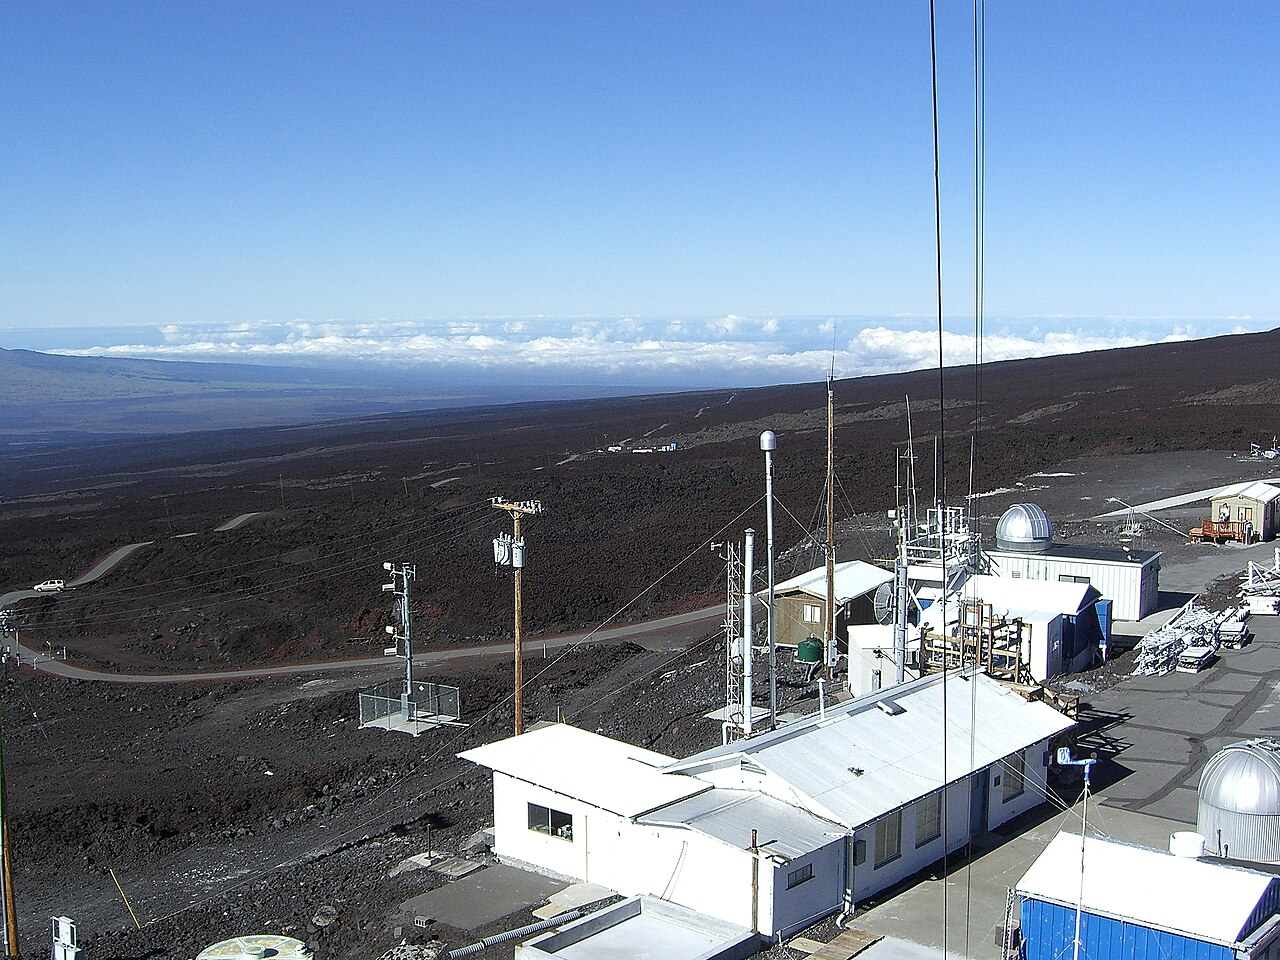
\includegraphics[width=0.56\linewidth]{images/book4/mauna-loa.jpg}\hspace{0.03\linewidth}
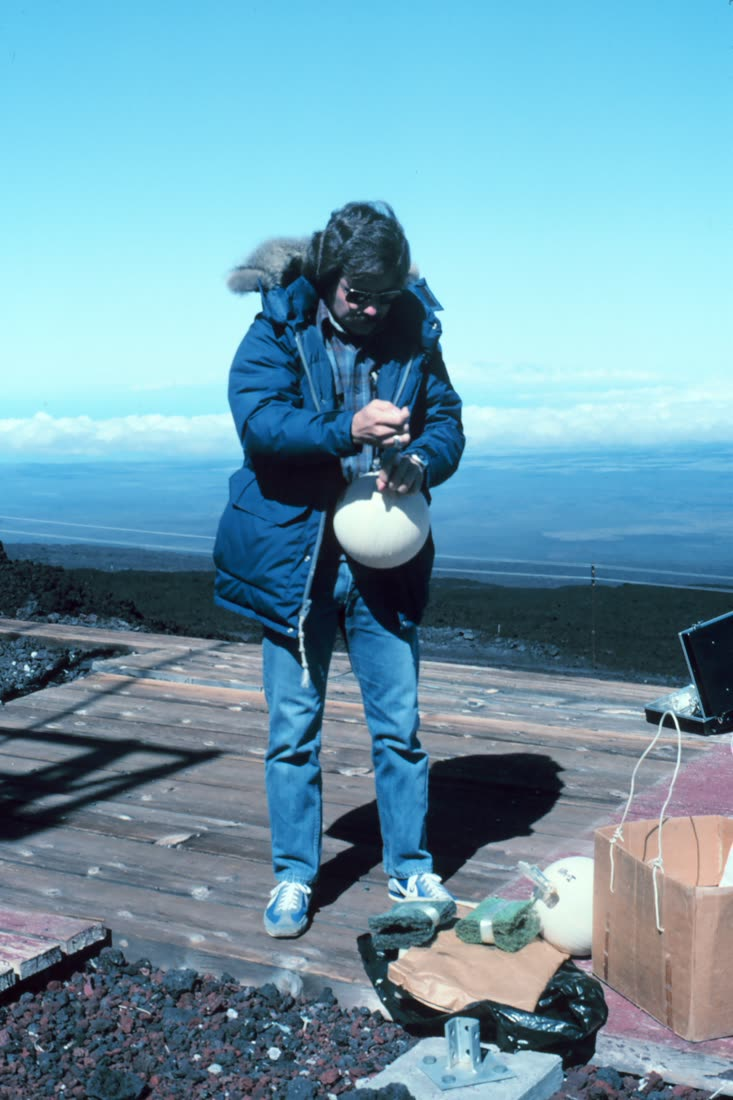
\includegraphics[width=0.33\linewidth]{images/book4/keeling-flask.jpg}

{\small वह वक्र कहाँ खींचा जाता है। बाएँ: मौना लोआ के उत्तरी
पार्श्व पर वह वेधशाला, \qty{3400}{m} ऊपर, उस व्यापारिक-पवन
व्युत्क्रमण के ऊपर जो उस द्वीप की अपनी वायु नीचे रखता है। दाएँ: 1982 में
लिया जाता कोई फ़्लास्क-नमूना; ऐसे फ़्लास्क, जिनका विश्लेषण
कैलिफ़ोर्निया में होता है, उस सतत विश्लेषक को जाँचते हैं और अलास्का से दक्षिणी ध्रुव तक
स्टेशनों पर भरे जाते हैं।}
\end{omfigure}

\section{नाइट्रोजन चक्र}

\begin{proposition}[नाइट्रोजन चक्र]\label{prop:b2:biogeochemical-cycles:nitrogen}
\index{नाइट्रोजन चक्र}\index{नाइट्रोजन स्थिरीकरण}\index{नाइट्रीकरण}\index{विनाइट्रीकरण}\index{हाबर--बॉश प्रक्रम}\index{ऐनैमॉक्स}
नाइट्रोजन प्रचुर है --- वायु $4\times 10^{9}$~Tg $\mathrm{N_2}$
थामे है --- और दुर्लभ भी, क्योंकि $\mathrm{N_2}$ का त्रिबंध
केवल दो प्रक्रमों से खुलता है: बिजली (वर्ष भर में कुछ Tg) और
प्रोकैरियोटों द्वारा नाइट्रोजनेज़ से \emph{जैविक \omterm{prop:b2:biogeochemical-cycles:nitrogen}{नाइट्रोजन स्थिरीकरण}},
यानी स्थल पर वर्ष भर में कोई 100 Tg और समुद्र में 100, और वह भी
प्रति $\mathrm{N_2}$ 16 ATP के दाम पर। स्थिर नाइट्रोजन फिर सूक्ष्मजीवों से
चलाई गई कोई अपचयोपचय सीढ़ी चलती है (\cref{ch:b2:microbial-metabolism}):
मृत पदार्थ का $\mathrm{NH_4^{+}}$ में \emph{अमोनीकरण};
वायवीय रसशिलापोषियों द्वारा $\mathrm{NH_4^{+}}$ का $\mathrm{NO_2^{-}}$ तथा $\mathrm{NO_3^{-}}$ में
\emph{नाइट्रीकरण}; पौधों द्वारा $\mathrm{NH_4^{+}}$ या $\mathrm{NO_3^{-}}$ का ग्रहण
और उनका वापस ऐमीन में अपचयन; और, जहाँ ऑक्सीजन न हो, वहाँ
$\mathrm{NO_3^{-}}$ का $\mathrm{N_2}$ में \emph{\omterm{def:b2:microbial-metabolism:anaerobic}{विनाइट्रीकरण}} ($\mathrm{N_2O}$ के किसी
रिसाव समेत) तथा \emph{ऐनैमॉक्स}, यानी नाइट्राइट से अमोनियम का
अवायवीय ऑक्सीकरण $\mathrm{N_2}$ में, जो मिलकर वायु को लगभग उतना ही लौटा देते हैं
जितना स्थिरीकरण लेता है। जीवमंडल में किसी नाइट्रोजन परमाणु का
\omterm{def:b2:biogeochemical-cycles:reservoir}{निवास-काल} कुछ सौ वर्ष है; और वायुमंडल में, $4\times
10^{9}/400 \approx 10^{7}$ वर्ष। 1913 से \emph{हाबर--बॉश}
प्रक्रम औद्योगिक रूप से नाइट्रोजन स्थिर करता आया है, अब वर्ष भर में लगभग 120 Tg,
और खेती की गई शिंबियाँ तथा जीवाश्म-ईंधन दहन 60 तथा 30 जोड़ते हैं:
मानवीय गतिविधि सारे प्राकृतिक प्रक्रमों जितनी ही नाइट्रोजन
मिलाकर स्थिर करती है, और जीवित आधे लोगों को खिलाती है।
\end{proposition}

\begin{omfigure}
\begin{tikzpicture}[every node/.style={font=\scriptsize}, >=stealth, box/.style={draw, rounded corners, minimum width=1.9cm, minimum height=0.8cm, align=center, fill=#1}]
  \node[box=omDef!15] (n2) at (0,3.4) {वायु में $\mathrm{N_2}$\\$4\times 10^{9}$ Tg};
  \node[box=omThm!15] (org) at (-4.6,1.0) {कार्बनिक N\\पौधे, मिट्टियाँ, समुद्र};
  \node[box=omProp!15] (nh4) at (-2.2,-0.8) {$\mathrm{NH_4^{+}}$};
  \node[box=omProp!15] (no2) at (2.2,-0.8) {$\mathrm{NO_2^{-}}$};
  \node[box=omProp!15] (no3) at (4.6,1.0) {$\mathrm{NO_3^{-}}$};
  \draw[->, thick] (n2) -- node[above left, align=right] {स्थिरीकरण\\नाइट्रोजनेज़, 200\\हाबर--बॉश 120} (org);
  \draw[->, thick] (org.south) -- node[below left] {अमोनीकरण} (nh4.north);
  \draw[->, thick] (nh4) -- node[below] {नाइट्रीकरण} (no2);
  \draw[->, thick] (no2) -- node[below right] {नाइट्रीकरण} (no3);
  \draw[->, thick] (no3) to[bend left=18] node[above, pos=0.72] {स्वांगीकरण} (org);
  \draw[->, thick, omExo!80!black] (no3) -- node[above right, align=left] {विनाइट्रीकरण\\(अनॉक्सी), $\mathrm{N_2O}$ रिसाव} (n2);
  \draw[->, thick, omExo!80!black] (no2) -- node[right, pos=0.55, align=left] {ऐनैमॉक्स\\($\mathrm{NH_4^{+}}$ के साथ)} (n2);
  \node[anchor=north, align=center] at (0,-1.5) {अभिवाह Tg N प्रति वर्ष में; स्वांगीकरण तथा अमोनीकरण को छोड़ हर चरण प्रोकैरियोट करते हैं};
\end{tikzpicture}

{\small अपचयोपचय सीढ़ी के रूप में \omterm{prop:b2:biogeochemical-cycles:nitrogen}{नाइट्रोजन चक्र} (पौधे नाइट्रेट के साथ
अमोनियम भी स्वांगीकृत करते हैं)। स्थिरीकरण तथा \omterm{def:b2:microbial-metabolism:anaerobic}{विनाइट्रीकरण}, यानी
वायुमंडल के दोनों द्वार, दोनों सूक्ष्मजीवीय हैं; और वह औद्योगिक द्वार
अब उस प्राकृतिक के बराबर है।}
\end{omfigure}

\begin{proof}[प्रमाण-सामग्री]
हबर्ड ब्रुक प्रायोगिक वन, न्यू हैंपशर: 1965 में एक
पूरा जल-विभाजक साफ़ काट दिया गया और शाकनाशी से नंगा रखा गया,
जबकि कोई पड़ोसी अक्षत छोड़ दिया गया, और हर एक से बहती धाराएँ
वर्षों तक मापी तथा विश्लेषित की गईं। उस उघाड़े जल-विभाजक ने
नियंत्रण की दर से साठ गुना नाइट्रेट खोया --- यानी मिट्टी की पूरी
नाइट्रोजन-पूँजी, जो अब पौधे नहीं ले रहे थे,
नाइट्रीकृत होकर बह गई, और अपने साथ कैल्सियम तथा पोटैशियम ले गई तथा
उस धारा को अम्लीय कर दिया। उस प्रयोग ने किसी अक्षत वन में उस चक्र की कसावट
(प्रति हेक्टेयर प्रति वर्ष कुछ किलोग्राम नाइट्रोजन की हानि,
सैकड़ों के चक्रित होने के मुक़ाबले) और उसे क्या तोड़ता है, दोनों दिखाए।
\end{proof}

\section{फ़ॉस्फ़ोरस और सल्फ़र}

\begin{proposition}[बिना किसी तेज़ गैस के दो चक्र]\label{prop:b2:biogeochemical-cycles:ps}
\index{फ़ॉस्फ़ोरस चक्र}\index{सल्फ़र चक्र}\index{सुपोषण}\index{डाइमेथिल सल्फ़ाइड}
\emph{फ़ॉस्फ़ोरस} का कोई गैसीय रूप नहीं है। वह पारिस्थितिकी-तंत्रों में
चट्टान में ऐपेटाइट के अपक्षय से घुसता है, यानी पूरी स्थल-सतह पर वर्ष भर में कोई 20 Tg,
मिट्टियों तथा झीलों के भीतर कई-कई बार पुनःचक्रित होता है
--- किसी झील के सतही जल में कोई फ़ॉस्फ़ेट आयन घंटों के भीतर
ले लिया जाता है --- और अवसादों को चला जाता है, जहाँ वह किसी
चट्टान-चक्र के $10^{8}$ वर्ष तक रहता है। इसलिए जीवन फ़ॉस्फ़ोरस-मितव्ययी
और फ़ॉस्फ़ोरस-सीमित है: महासागर में \omterm{def:b2:biogeochemical-cycles:reservoir}{निवास-काल} कोई
\num{20000} वर्ष है, और गहरे समुद्र का फ़ॉस्फ़ेट, जो
उत्प्लवन से ऊपर लाया जाता है, उसकी उत्पादकता बाँधता है। खनन अब
खेती की ज़मीन पर लगभग उतना ही फ़ॉस्फ़ोरस चलाता है जितना अपक्षय छोड़ता है, और झीलों में उसका
बहाव \emph{सुपोषण} करता है: यानी कोई शैवाल-प्रस्फुटन, उसका क्षय,
ऑक्सीजन की खपत, और मछलियों की मौत --- 1970 के दशक में ओंटारियो में
शिंडलर के पूरी-झील प्रयोगों ने, जिनमें किसी झील का एक आधा भाग
फ़ॉस्फ़ोरस से उर्वरित किया गया और दूसरा नहीं, दिखाया कि केवल फ़ॉस्फ़ोरस ही
वह प्रवर्तक है, और उन्होंने उसे अपमार्जकों से हटवा दिया।
\emph{सल्फ़र} का चट्टान-चक्र (जिप्सम, पाइराइट) भी है और कोई
गैस-प्रावस्था भी: यानी ज्वालामुखियों तथा कोयले की $\mathrm{SO_2}$, अनॉक्सी
अवसादों की $\mathrm{H_2S}$, और समुद्री प्लवक से \emph{\omterm{prop:b2:biogeochemical-cycles:ps}{डाइमेथिल सल्फ़ाइड}}, जिसके
ऑक्सीकरण-उत्पाद महासागर के ऊपर बादलों के बीज बनते हैं। कोयला जलाने ने
बीसवीं सदी में वायु तक सल्फ़र का \omterm{def:b2:biogeochemical-cycles:reservoir}{अभिवाह} तिगुना कर दिया और
यूरोप तथा उत्तरी अमेरिका को उनकी अम्ल-वर्षा दी; और स्क्रबरों ने उसे
दशकों के भीतर उलट दिया, क्योंकि वायु में उस चक्र का \omterm{def:b2:biogeochemical-cycles:reservoir}{निवास-काल}
कुछ ही दिन है।
\end{proposition}

\begin{omfigure}
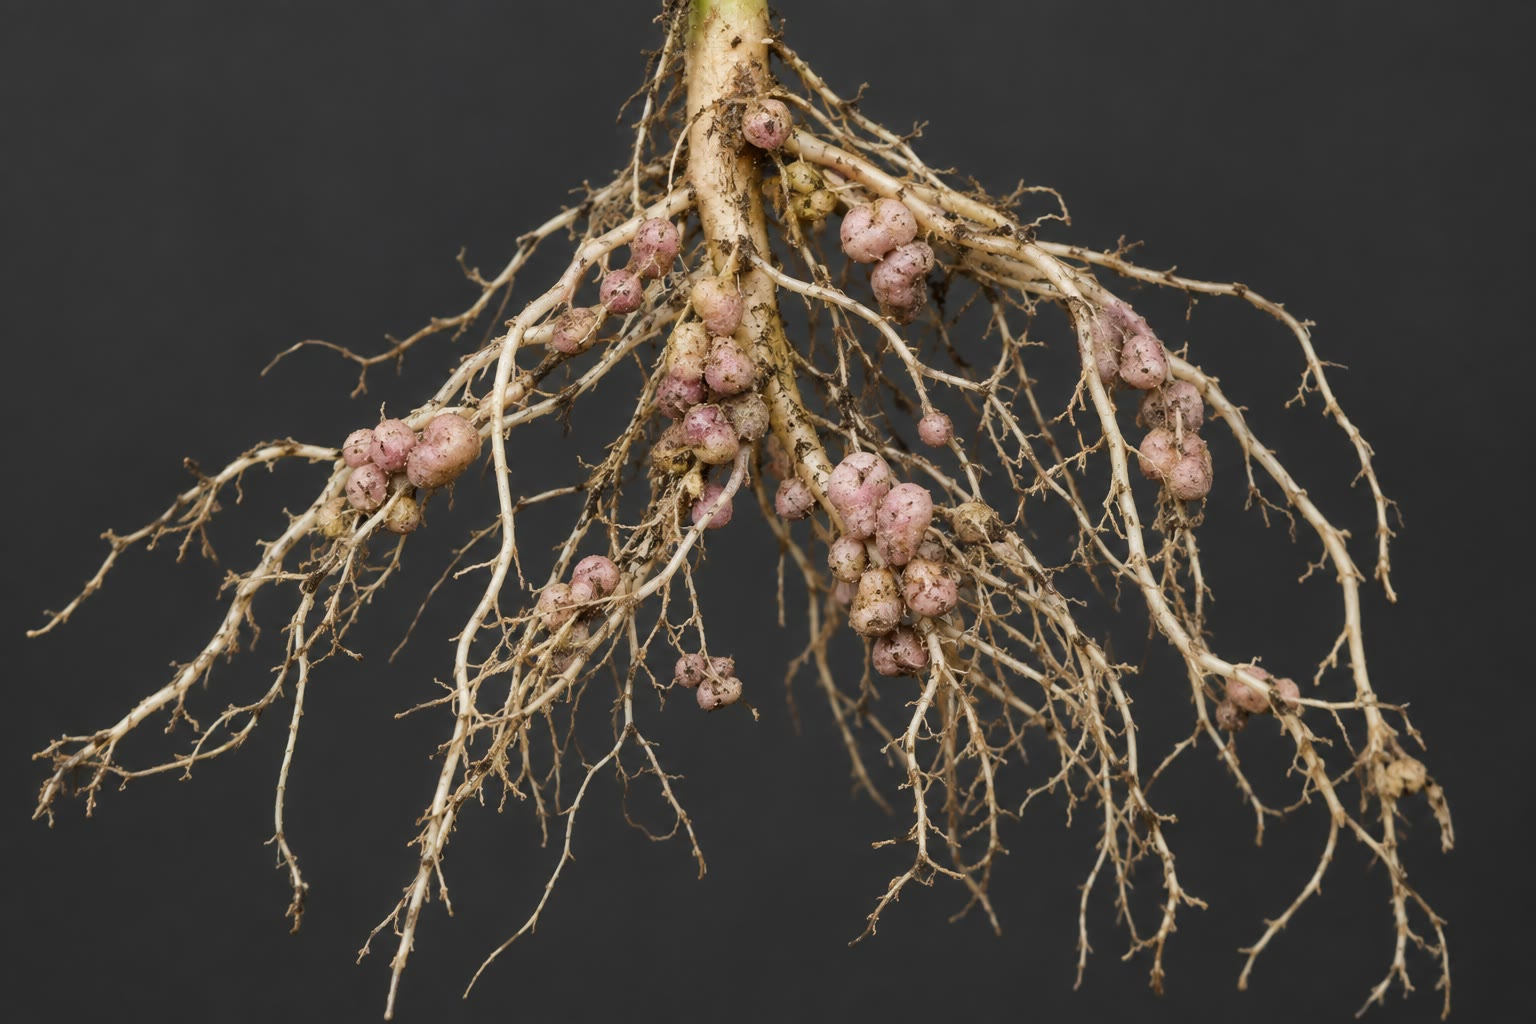
\includegraphics[width=0.44\linewidth]{images/book4/ai/b4-25-root-nodules.jpg}\hspace{0.04\linewidth}
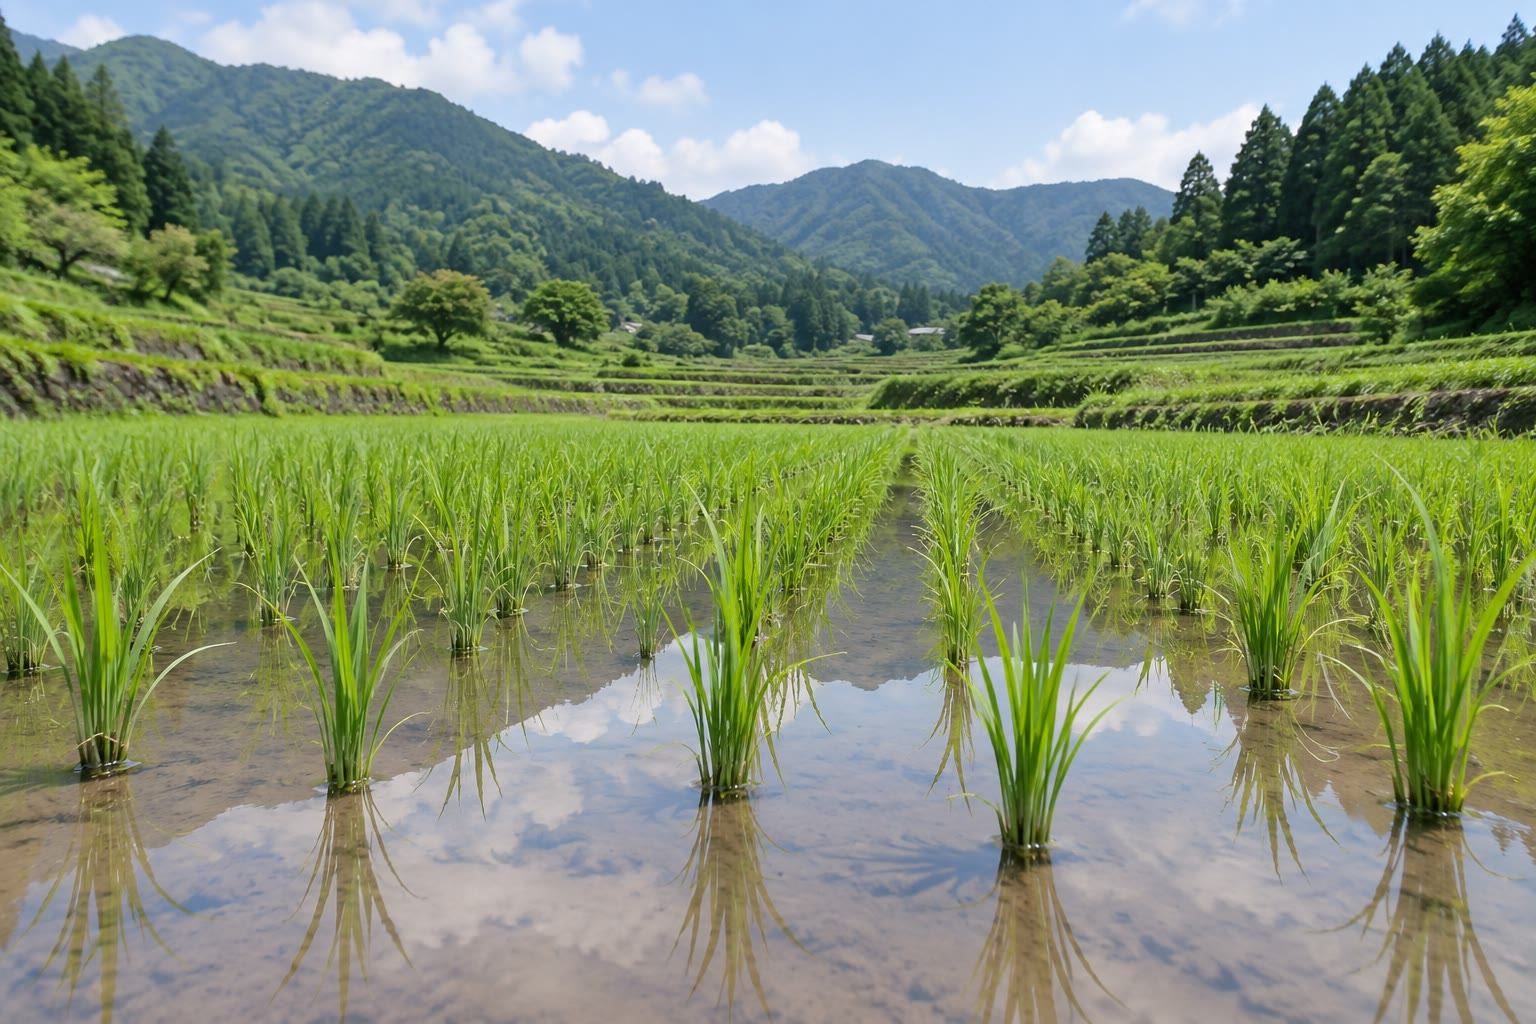
\includegraphics[width=0.44\linewidth]{images/book4/ai/b4-25-rice-paddy.jpg}

{\small \omterm{prop:b2:biogeochemical-cycles:nitrogen}{नाइट्रोजन चक्र} के दो द्वार। बाएँ: किसी शिंबी की मूल-ग्रंथिकाएँ,
हर एक कोई कक्ष जिसमें राइजोबिया अपने परपोषी के लिए नाइट्रोजन स्थिर
करते हैं। दाएँ: कोई जलमग्न धान का खेत, सतह के नीचे अनॉक्सी, जहाँ
\omterm{def:b2:microbial-metabolism:anaerobic}{विनाइट्रीकरण} नाइट्रोजन को वायु में लौटाता है और मीथेनजन
मीथेन बनाते हैं।}
\end{omfigure}

\section{विक्षुब्ध ग्रह}

\begin{example}[वे अंक क्या कहते हैं]\label{ex:b2:biogeochemical-cycles:numbers}
$0.45$ के किसी \omterm{prop:b2:biogeochemical-cycles:carbon}{वायुवाहित अंश} के साथ वर्ष भर में \qty{10}{GtC} का उत्सर्जन
हर वर्ष वायु में \qty{4.5}{GtC}, यानी \qty{2.1}{ppm}, छोड़ जाता है
--- यानी वही देखी गई ढाल। 1850 से संचयी उत्सर्जन लगभग
\qty{700}{GtC} हैं, जिनमें से \qty{290}{GtC} वायु में है (140~ppm), और
बाक़ी महासागर तथा स्थल में। वायुमंडल को किसी भी स्तर पर थामने के लिए शुद्ध
उत्सर्जन गिरकर उतने होने चाहिए जितने वे धीमे पात्र --- गहरे-महासागर का मिश्रण तथा
अपक्षय, जो मिलकर वर्ष भर में \qty{1}{GtC} से कम हैं --- ले सकें:
\emph{शुद्ध शून्य} कोई नारा नहीं बल्कि बहुत लंबे $\tau$ के साथ उस \omterm{thm:b2:biogeochemical-cycles:box}{डिब्बा-प्रतिरूप} की
स्थायी-अवस्था शर्त है। नाइट्रोजन के लिए,
स्थिर-नाइट्रोजन \omterm{def:b2:biogeochemical-cycles:reservoir}{अभिवाह} के दुगुने होने ने नदियों में नाइट्रेट दुगुना कर दिया है,
मिसिसिपी तथा बाल्टिक के मुहानों पर मृत क्षेत्र पैदा किए हैं, और
वायुमंडल की $\mathrm{N_2O}$, जो शताब्दी भर के \omterm{def:b2:biogeochemical-cycles:reservoir}{निवास-काल} वाली कोई
हरितगृह गैस है, पाँचवें भाग भर चढ़ा दी है। \Cref{ch:b2:global-change}
जीवों के लिए उसके परिणाम पीछा करता है।
\end{example}

\section{अभ्यास}

\begin{exercise}[$\star$]\label{exo:b2:biogeochemical-cycles:1}
\omterm{def:b2:biogeochemical-cycles:reservoir}{भंडार}, \omterm{def:b2:biogeochemical-cycles:reservoir}{अभिवाह} तथा \omterm{def:b2:biogeochemical-cycles:reservoir}{निवास-काल} की परिभाषा दीजिए, और
स्थल-पौधों में (450 GtC, प्रकाशसंश्लेषण वर्ष भर में
120 GtC) तथा गहरे महासागर में (\num{37000} GtC, विनिमय
वर्ष भर में लगभग 100 GtC) कार्बन का \omterm{def:b2:biogeochemical-cycles:reservoir}{निवास-काल} निकालिए।
\end{exercise}

\begin{exercise}[$\star$]\label{exo:b2:biogeochemical-cycles:2}
वर्ष भर में \qty{2.5}{ppm} को GtC में, और \qty{10}{GtC} उत्सर्जन को
ppm में बदलिए।
\end{exercise}

\begin{exercise}[$\star$]\label{exo:b2:biogeochemical-cycles:3}
वे दो प्राकृतिक प्रक्रम बताइए जो $\mathrm{N_2}$ खोलते हैं, वह प्रक्रम जो उसे
लौटाता है, और बीच के तीनों अपचयोपचय चरण, और हर एक के लिए
ज़िम्मेदार जीव।
\end{exercise}

\begin{exercise}[$\star$]\label{exo:b2:biogeochemical-cycles:4}
भूवैज्ञानिक समय पर फ़ॉस्फ़ोरस नाइट्रोजन से अधिक बार उत्पादकता क्यों
सीमित करता है, और किसी दी गई ऋतु में नाइट्रोजन फ़ॉस्फ़ोरस से अधिक बार
क्यों?
\end{exercise}

\begin{exercise}[$\star\star$]\label{exo:b2:biogeochemical-cycles:5}
\qty{e7}{m^3} की कोई झील वर्ष भर में \qty{2}{t} फ़ॉस्फ़ोरस पाती है
और अपने जल का \qty{20}{\%} वार्षिक रूप से बहा देती है। उसकी स्थायी-अवस्था
फ़ॉस्फ़ोरस सांद्रता और उस निवेश के शुरू होने के बाद उसका \qty{90}{\%}
पाने का काल निकालिए। यदि वह निवेश आधा हो जाए तो?
\end{exercise}

\begin{exercise}[$\star\star$]\label{exo:b2:biogeochemical-cycles:6}
कीलिंग आँकड़ों से 1960 के दशक में (दस वर्षों में 316 से \qty{325}{ppm})
और 2010 के दशक में (नौ वर्षों में 390 से 411) $\mathrm{CO_2}$ की
माध्य वृद्धि-दर वर्ष भर में ppm में तथा वर्ष भर में GtC में निकालिए।
\end{exercise}

\begin{exercise}[$\star\star$]\label{exo:b2:biogeochemical-cycles:7}
मौना लोआ पर ऋतुई आरे-दाँत का आयाम शिखर से गर्त तक लगभग
\qty{6}{ppm} है। उसे GtC में बदलिए और उत्तरी गोलार्ध के स्थल के
वार्षिक शुद्ध प्राथमिक उत्पादन, यानी लगभग \qty{35}{GtC}, से तुलना कीजिए। वह आरा-दाँत इतना छोटा क्यों है?
\end{exercise}

\begin{exercise}[$\star\star$]\label{exo:b2:biogeochemical-cycles:8}
नाइट्रोजनेज़ प्रति $\mathrm{N_2}$ 16 ATP ख़र्च करता है। प्रति हेक्टेयर प्रति वर्ष
\qty{200}{kg} नाइट्रोजन स्थिर करती किसी शिंबी के लिए, स्थिर
$\mathrm{N_2}$ के मोल तथा ख़र्च हुई ATP, और वह ग्लूकोज़-द्रव्यमान निकालिए जो वह ATP
दर्शाती है (प्रति ग्लूकोज़ लगभग 30 ATP)। वह किसी
\qty{10}{t/ha} फ़सल के प्रकाशसंश्लिष्ट का कौन-सा अंश है?
\end{exercise}

\begin{exercise}[$\star\star$]\label{exo:b2:biogeochemical-cycles:9}
प्लवक रेडफ़ील्ड अनुपात $\mathrm{C:N:P} = 106:16:1$ पर बढ़ते हैं।
गहराई पर समुद्री जल \qty{2.2}{\micro mol/kg} फ़ॉस्फ़ेट तथा
\qty{32}{\micro mol/kg} नाइट्रेट थामे है। किसी पिंड को सतह पर लाने पर
कौन-सा पहले चुकता है, और उससे पहले कितना कार्बन स्थिर
होता है?
\end{exercise}

\begin{exercise}[$\star\star\star$]\label{exo:b2:biogeochemical-cycles:10}
वायुमंडल को ऐसे किसी डिब्बे की तरह लीजिए जिसका अतिरिक्त कार्बन $E$ उन पात्रों से
दर $E/\tau$ पर हटाया जाता है और जिसे उत्सर्जन $Q$ पोसते हैं। $\tau =
50$ वर्ष तथा $Q = \qty{10}{GtC/yr}$ के साथ, स्थायी-अवस्था
अतिरेक क्या है और वह किस ppm के अनुरूप है? समझाइए कि असली
उत्तर उससे बुरा क्यों है।
\end{exercise}

\begin{exercise}[$\star\star\star$]\label{exo:b2:biogeochemical-cycles:11}
बम-परीक्षणों ने 1963 में वायुमंडल की $\mathrm{{}^{14}C}$ दुगुनी कर दी; वह
अतिरेक फिर कोई 11 वर्षों में आधा होता गया, जबकि $\mathrm{{}^{14}C}$
की अर्ध-आयु 5730 वर्ष है। समझाइए कि क्या मापा गया, और
वे 11 वर्ष आपको \omterm{prop:b2:biogeochemical-cycles:carbon}{कार्बन चक्र} के बारे में क्या बताते हैं।
\end{exercise}

\begin{exercise}[$\star\star\star$]\label{exo:b2:biogeochemical-cycles:12}
``मनुष्यों ने \omterm{prop:b2:biogeochemical-cycles:nitrogen}{नाइट्रोजन चक्र} दुगुना कर दिया है और \omterm{prop:b2:biogeochemical-cycles:carbon}{कार्बन चक्र}
को केवल ठेला है।'' अंकों के साथ इस पर विचार कीजिए: स्थिर किए गए \omterm{def:b2:biogeochemical-cycles:reservoir}{अभिवाह}, प्राकृतिक
\omterm{def:b2:biogeochemical-cycles:reservoir}{अभिवाह} के अंश, और प्रभावित \omterm{def:b2:biogeochemical-cycles:reservoir}{भंडार}।
\end{exercise}

\section{समस्या: किसी सदी का कार्बन बजट}

\begin{problem}[{सप्तांत समस्या --- सदी भर के उत्सर्जन
वायुमंडल के डिब्बा-प्रतिरूप से गुज़ारे गए, महासागर का हिस्सा
तथा स्थल का, किसी उर्वरित खेत से किसी मृत क्षेत्र तक नाइट्रोजन-झरना, और किसी
झील का फ़ॉस्फ़ोरस बजट, और अंत उस वायुवाहित
अंश, 2100 में वायुमंडलीय सांद्रता, तथा प्रति हेक्टेयर खोई गई
नाइट्रोजन पर}]
\label{pb:b2:biogeochemical-cycles:1}
आँकड़े। 1850 में वायुमंडल: \qty{285}{ppm}; \qty{1}{ppm} $=
\qty{2.13}{GtC}$। 1850--2020 के संचयी उत्सर्जन: \qty{700}{GtC};
2020 में वायुमंडलीय $\mathrm{CO_2}$: \qty{412}{ppm}। \qty{1}{ha} का कोई खेत
वर्ष भर में \qty{150}{kg} नाइट्रोजन उर्वरक पाता है;
वह फ़सल \qty{60}{\%} लेती है, \qty{25}{\%} विनाइट्रीकृत होता है, और
बाक़ी बह जाता है। \qty{5e7}{m^3} की कोई झील वर्ष भर में अपने जल का दसवाँ भाग
बहा देती है और वर्ष भर में \qty{5}{t} फ़ॉस्फ़ोरस पाती है।

\medskip
\noindent\textbf{भाग I --- वह \omterm{prop:b2:biogeochemical-cycles:carbon}{वायुवाहित अंश}।}
\begin{enumerate}
  \item 1850 में तथा 2020 में वायुमंडलीय कार्बन, और GtC में वह
        वृद्धि निकालिए।
  \item 1850--2020 भर \omterm{prop:b2:biogeochemical-cycles:carbon}{वायुवाहित अंश} निकालिए।
  \item बाक़ी कहाँ है? उस प्रतिज्ञप्ति से वे दो पात्र और उनके
        अनुमानित हिस्से दीजिए।
  \item यदि महासागर ने उन उत्सर्जनों का \qty{25}{\%} लिया हो, तो उसका
        घुला अकार्बनिक कार्बन, \qty{38000}{GtC}, सापेक्ष रूप से कितना
        चढ़ा है? फिर भी वह सतही महासागर मापने लायक ढंग से
        अम्लीय क्यों होता है?
  \item उत्सर्जनों के चरघातांकी रूप से बढ़ने पर भी वह \omterm{prop:b2:biogeochemical-cycles:carbon}{वायुवाहित अंश}
        मोटे तौर पर अचल क्यों रहता है? ($Q \propto e^{t/T}$ तथा
        किसी पात्र $E/\tau$ के साथ उस \omterm{thm:b2:biogeochemical-cycles:box}{डिब्बा-प्रतिरूप} पर विचार कीजिए।)
  \item यदि उत्सर्जन बहुत शताब्दियों तक अचल रखे जाएँ तो वह
        \omterm{prop:b2:biogeochemical-cycles:carbon}{वायुवाहित अंश} क्या हो जाता?
\end{enumerate}

\medskip
\noindent\textbf{भाग II --- आने वाली सदी।}
अतिरिक्त कार्बन $E$ (1850 के स्तर से ऊपर) को
$\mathrm{d}E/\mathrm{d}t = Q - E/\tau$, $\tau = 100$ वर्ष से प्रतिरूपित कीजिए।
\begin{enumerate}[resume]
  \item 2020 में अतिरेक GtC में निकालिए।
  \item $Q$ को \qty{10}{GtC/yr} पर थामकर स्थायी-अवस्था
        अतिरेक और वह सांद्रता निकालिए जो वह सुझाता है।
  \item 2020 से $E(t)$ हल कीजिए, $Q = 10$ के साथ, और 2100 में $E$
        तथा वह सांद्रता दीजिए।
  \item अब $Q$ को 2020 तथा 2070 के बीच रैखिक रूप से शून्य तक गिरने दीजिए और
        शून्य पर रहने दीजिए। 2070 में तथा 2100 में $E$ निकालिए (उस समीकरण का
        समाकलन कीजिए; किसी रैखिक $Q$ के लिए विशेष हल रैखिक धन कोई
        अचरांक है)।
  \item 2100 की दोनों सांद्रताओं की तुलना कीजिए।
  \item दूसरे परिदृश्य के लिए कोई एक ही $\tau$ आशावादी क्यों है?
\end{enumerate}

\medskip
\noindent\textbf{भाग III --- नाइट्रोजन-झरना।}
\begin{enumerate}[resume]
  \item प्रति हेक्टेयर प्रति वर्ष फ़सल से ली गई, विनाइट्रीकृत तथा
        बही हुई नाइट्रोजन निकालिए।
  \item वह बही हुई नाइट्रोजन किसी नदी तक नाइट्रेट के रूप में पहुँचती है और फिर उस
        समुद्र तक, जहाँ प्लवक उसे रेडफ़ील्ड अनुपात पर काम में लेते हैं। वह प्लवक को कितना
        कार्बन स्थिर करने देती है?
  \item वह कार्बन डूबता है और गहराई पर श्वसित होता है, और
        प्रति C 1 $\mathrm{O_2}$ पर ऑक्सीजन खपाता है। खपी ऑक्सीजन
        मोलों में तथा किलोग्रामों में निकालिए।
  \item समुद्री जल का कोई घन मीटर संतृप्त होने पर लगभग \qty{0.25}{mol}
        $\mathrm{O_2}$ थामे है। एक हेक्टेयर का बहाव तली के जल के कितने घन मीटर
        निर्ऑक्सीजनित करता है?
  \item वह विनाइट्रीकृत अंश आंशिक रूप से $\mathrm{N_2O}$ के रूप में निकल जाता है, यानी
        विनाइट्रीकृत नाइट्रोजन का \qty{1}{\%}। प्रति हेक्टेयर प्रति वर्ष $\mathrm{N_2O}$,
        और $\mathrm{CO_2}$ में उसका तापन-तुल्यांक निकालिए
        ($\mathrm{N_2O}$ प्रति किलोग्राम $\mathrm{CO_2}$ से 270 गुना है)।
  \item उस $\mathrm{CO_2}$ से तुलना कीजिए जो वह उर्वरक बनाने में उत्सर्जित हुई
        (हाबर--बॉश से प्रति किलोग्राम नाइट्रोजन लगभग \qty{4}{kg}
        $\mathrm{CO_2}$)।
\end{enumerate}

\medskip
\noindent\textbf{भाग IV --- वह झील।}
\begin{enumerate}[resume]
  \item यदि एकमात्र हानि बहाव हो तो उस झील का फ़ॉस्फ़ोरस \omterm{def:b2:biogeochemical-cycles:reservoir}{निवास-काल},
        और उसकी स्थायी-अवस्था सांद्रता
        \unit{mg/m^3} में निकालिए।
  \item \qty{30}{mg/m^3} से अधिक फ़ॉस्फ़ोरस वाली झीलें
        सुपोषी हैं। क्या यह है?
  \item अवसादन 5 वर्ष के अपने ही काल-नियतांक से फ़ॉस्फ़ोरस हटाता है।
        वह \omterm{def:b2:biogeochemical-cycles:reservoir}{निवास-काल} तथा वह सांद्रता फिर से
        निकालिए।
  \item वह निवेश घटाकर वर्ष भर में \qty{1}{t} कर दिया जाता है। नई
        \omterm{def:b2:biogeochemical-cycles:reservoir}{स्थायी अवस्था} और उसके \qty{10}{\%} के भीतर पहुँचने का काल निकालिए।
  \item बहुत-सी झीलें इस गणना के बताए से अधिक धीरे क्यों
        उबरती हैं?
  \item उस \qty{5}{t} निवेश से रेडफ़ील्ड अनुपात पर वह कार्बन निकालिए
        जिसे उस झील का फ़ॉस्फ़ोरस हर वर्ष प्लवक में बना सकता है।
  \item परिणाम बताइए: वह \omterm{prop:b2:biogeochemical-cycles:carbon}{वायुवाहित अंश}, 2100 की दोनों
        सांद्रताएँ, और प्रति हेक्टेयर बही हुई
        नाइट्रोजन।
\end{enumerate}
\end{problem}
